\chapter{Introdução}

As metodologias ágeis vem ganhando cada vez espaço no mercado global 
de desenvolvimento de software, pois enfatizam a qualidade do produto 
sobre a qualidade do processo, procurando minimizar a execução 
de atividades não essenciais ao longo do ciclo de vida de 
desenvolvimento de software. 

O eXtreme Programming (XP), que é uma metodologia ágil, tem a codificação como a 
atividade chave durante um projeto de software \cite{beck1999}. Isso também se 
torna perceptível por algumas práticas do 
XP~\footnote{Documentação disponível em \url{http://www.extremeprogramming.org}}
 :

\begin{enumerate}
%-----------------------------
\item Padronização do Código: O código é a principal forma de comunicação entre 
a equipe, logo a padronização de código o torna consistente e fácil para todo o 
time ler e refatorar. 
%-----------------------------
\item Propriedade Coletiva do Código: Cada programador pode melhorar qualquer 
parte do código quando existir a oportunidade.
%-----------------------------
\item Programação em Pares: Todo código é escrito com duas pessoas: uma que olha 
para uma máquina, e outra com um teclado e um mouse.
%-----------------------------
\item Integração Contínua: Todo novo código é integrado ao sistema e quando 
integrado, o sistema é totalmente reconstruído do zero e todos os testes devem 
passar ou o novo código é descartado.

\end{enumerate} 


Logo em metodologias ágeis, é possível inferir a qualidade do trabalho 
desenvolvido, por meio do código-fonte. Um dos métodos mais utilizados é a 
análise estática de código, o qual segundo \citeonline{Emanuelsson2008} 
significa método automático de coleta de propriedades de tempo de execução do 
código-fonte sem executá-lo e os resultados da análise podem servir para 
propósitos de verificação de erros, geração automática de casos de teste, 
análise de impacto ou ainda para obtenção de métricas de código-fonte.

Embora a definição formal da análise estática consolidada no âmbito acadêmico, 
vide os trabalhos de \cite{Wichmann95} e \cite{Nielson:1999}, as ferramentas 
disponíveis no mercado, que realizam as coletas e avaliação, 
ainda não suprem totalmente as necessidades de quem precisa avaliar a 
qualidade total do produto.

Este fato ocorre, pois as ferramentas apresentam os seguintes problemas:

\newlist{myList}{enumerate}{3}
\setlist[myList]{ label* = P\arabic* -}

\begin{myList}
    \item Ausência de resultados consolidados do produto, pois a maior 
	parte das métricas é extraída de elementos internos menores (Bibliotecas, 
	Pacotes, Classes,Métodos, Funções).
    
	\item Ausência de mecanismos de tratamento, separação, recuperação e 
	organização e persistência de dados. 
	
	\item Ausência de associação entre resultados numéricos e forma de 
	interpretá-los: Ferramentas de análise estática frequentemente mostram 
	seus resultados como valores numéricos isolados para cada métrica 
	\cite{Meirelles2013}. 
	
	\item Em grande parte das ferramentas, a visualização dos resultados não é 
	agradável, isto é, são apresentados um conjunto de dados em uma janela 
	terminal contendo os valores das métricas.
	
    \end{myList}
	
	

%------------------------------------------------------------------------------%





%------------------------------------------------------------------------------%

\section{Objetivos}

Esta seção apresenta os objetivos gerais e específicos deste TCC.

\subsection{Objetivos Gerais}
Sob prisma da avaliação da qualidade de código em ambientes ágeis, 
neste trabalho, há como objetivo geral a proposição e construção um ambiente de 
\textit{Dwing}, de modo a melhorar extração e visualização das métricas de 
código-fonte, suprimindo os pontos fracos enunciados acima das ferramentas de 
análise estática de código.

Este ambiente inicialmente construído para este trabalho de conclusão de curso, 
poderá ser expandido em trabalhos futuros para a coleta, transformação e 
correlação com outras métricas coletadas durante o processo de desenvolvimento 
de software. 


%------------------------------------------------------------------------------%

\subsection{Objetivos Específicos}

Os objetivos específicos desse trabalho são:

\begin{enumerate}
	
\item Construir o ambiente de Dwing para extração e visualização de métricas de 
código-fonte.
\item Incorporar indicadores qualitativos para cada métrica de código-fonte.
\item Facilitar o entendimento das métricas de código-fonte.

\end{enumerate}

%------------------------------------------------------------------------------%

\section{Sobre o Trabalho}
%------------------------------------------------------------------------------%
\subsection {Metodologia de Pesquisa}
A metodologia de pesquisa foi definida em:

\begin{description}

\item[Aplicada:] pois visa construir conhecimento para aplicações práticas 
dirigidos á solução de problemas específicos \cite{Gil2008}.

\item[Metodológica]

\end{description}

\subsection{Cronograma}
O Trabalho de Conclusão de Curso foi planejado, como um planejamento de 
longo prazo, em quatro ciclos de desenvolvimento de vinte e um dias. 
As figuras \ref{cronograma} e \ref{gantt}, que foram extraídas do 
OpenProj\footnote{\url{http://sourceforge.net/projects/openproj/}}, 
apresentam o cronograma geral o gráfico de Gantt do presente trabalho.

\begin{figure}[h]
\centering
	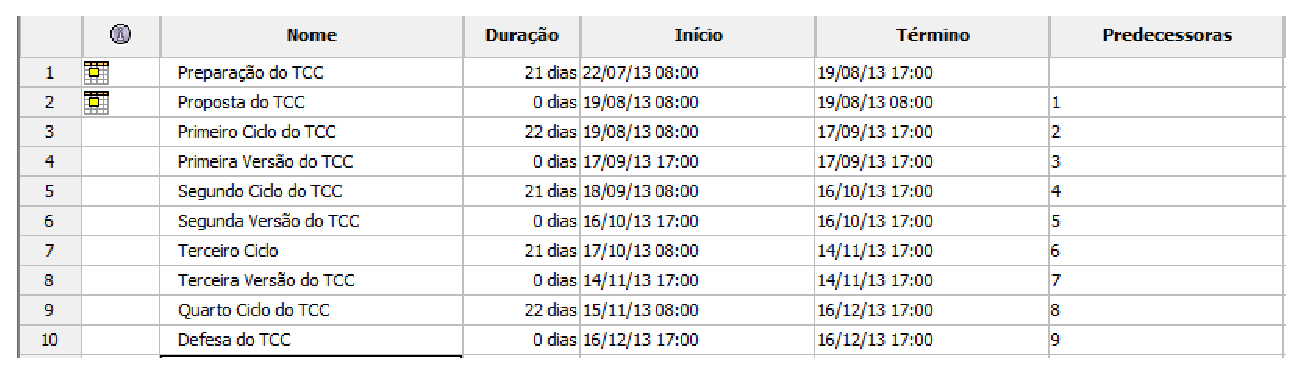
\includegraphics[keepaspectratio=true,scale=0.7]{figuras/marcos.eps}
	\caption{Ciclos de Desenvolvimento do Trabalho de Conclusão de Curso}
	\label{cronograma}
\end{figure}

\begin{figure}[h]
\centering
	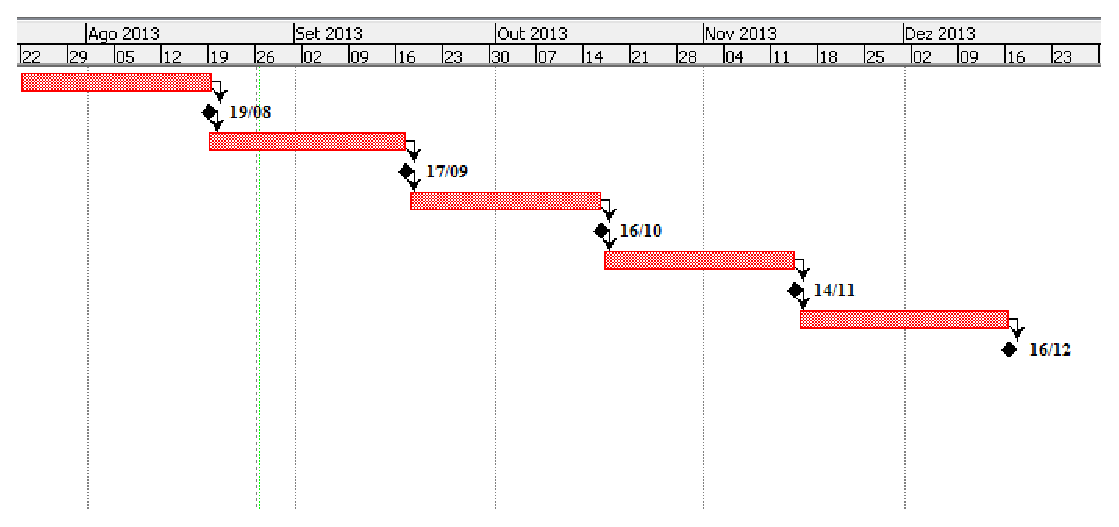
\includegraphics[keepaspectratio=true,scale=0.7]{figuras/gantt_chart.eps}
	\caption{Gráfico de Gantt}
	\label{gantt}
\end{figure}

Para cada ciclo de desenvolvimento do Trabalho de Conclusão de Curso,  
utilizou-se o Quadro \textit{Kanban}  



\subsection{Organização do Trabalho}
Para a primeira fase deste Trabalho de Conclusão de Curso, além desta introdução 
este texto está organizado em capítulos. O Capítulo 2 apresenta  o processo de 
medição e as métricas de código-fonte.
O Capítulo 3 apresenta o SonarQube como a ferramenta escolhida para extração das 
métricas de código-fonte.
O Capítulo 4 apresenta a fundamentação teórica do ambiente de Dwing, de modo a 
suprir as limitações das ferramentas, e cada um de seus componentes em detalhes. 
O Capítulo 5 apresenta o ambiente proposto por este trabalho para extração e 
visualização das métricas de código-fonte. Por fim, o Capítulo 6 apresenta o 
estado atual da validação 
do ambiente por meio de estudo de caso, bem como as atividades planejadas até o 
encerramento do trabalho de conclusão de curso.
